%%%%%%%%%%%%%%%%%%%%%%%%%%%%%%%%%%%%%%%%%
% Journal Article
% LaTeX Template
% Version 1.4 (15/5/16)
%
% This template has been downloaded from:
% http://www.LaTeXTemplates.com
%
% Original author:
% Frits Wenneker (http://www.howtotex.com) with extensive modifications by
% Vel (vel@LaTeXTemplates.com)
%
% License:
% CC BY-NC-SA 3.0 (http://creativecommons.org/licenses/by-nc-sa/3.0/)
%
%%%%%%%%%%%%%%%%%%%%%%%%%%%%%%%%%%%%%%%%%

%----------------------------------------------------------------------------------------
%	PACKAGES AND OTHER DOCUMENT CONFIGURATIONS
%----------------------------------------------------------------------------------------

\documentclass[twoside,twocolumn]{article}

\usepackage{blindtext} % Package to generate dummy text throughout this template 

\usepackage[sc]{mathpazo} % Use the Palatino font
\usepackage[T1]{fontenc} % Use 8-bit encoding that has 256 glyphs
\linespread{1.05} % Line spacing - Palatino needs more space between lines
\usepackage{microtype} % Slightly tweak font spacing for aesthetics

\usepackage[english]{babel} % Language hyphenation and typographical rules

\usepackage[hmarginratio=1:1,top=32mm,columnsep=20pt]{geometry} % Document margins
\usepackage[hang, small,labelfont=bf,up,textfont=it,up]{caption} % Custom captions under/above floats in tables or figures
\usepackage{booktabs} % Horizontal rules in tables

\usepackage{lettrine} % The lettrine is the first enlarged letter at the beginning of the text

\usepackage{enumitem} % Customized lists
\setlist[itemize]{noitemsep} % Make itemize lists more compact

\usepackage{abstract} % Allows abstract customization
\renewcommand{\abstractnamefont}{\normalfont\bfseries} % Set the "Abstract" text to bold
\renewcommand{\abstracttextfont}{\normalfont\small\itshape} % Set the abstract itself to small italic text

\usepackage{titlesec} % Allows customization of titles
\renewcommand\thesection{\Roman{section}} % Roman numerals for the sections
\renewcommand\thesubsection{\roman{subsection}} % roman numerals for subsections
\titleformat{\section}[block]{\large\scshape\centering}{\thesection.}{1em}{} % Change the look of the section titles
\titleformat{\subsection}[block]{\large}{\thesubsection.}{1em}{} % Change the look of the section titles

\usepackage{fancyhdr} % Headers and footers
\pagestyle{fancy} % All pages have headers and footers
\fancyhead{} % Blank out the default header
\fancyfoot{} % Blank out the default footer
\fancyhead[C]{Running title $\bullet$ May 2016 $\bullet$ Vol. XXI, No. 1} % Custom header text
\fancyfoot[RO,LE]{\thepage} % Custom footer text

\usepackage{titling} % Customizing the title section

\usepackage{hyperref} % For hyperlinks in the PDF

\usepackage{graphicx}

%----------------------------------------------------------------------------------------
%	TITLE SECTION
%----------------------------------------------------------------------------------------

\setlength{\droptitle}{-4\baselineskip} % Move the title up

\pretitle{\begin{center}\Huge\bfseries} % Article title formatting
\posttitle{\end{center}} % Article title closing formatting
\title{Report on the evolution of cooperation in relation to game-theory and different game-theoretic mechanisms to aid it} % Article title
\author{%
\textsc{James King} \\% Your name
\normalsize Supervisor: Kostas Stathis \\ % Your supervisor
}
\date{October 2018} % Leave empty to omit a date
\renewcommand{\maketitlehookd}{%
\begin{abstract}
\noindent Since the early days of Darwinian evolutionary theory the phrase ``Survival of the fittest" has become synonymous with much thinking on evolutionary dynamics. This idea has come along way since then but is still seen by many to promote selfish attitudes. However, we can see throughout nature that cooperation between biological agents is prevalent. So how did cooperation evolve and why has it flourished? This question fundamentally challenges what seemed concrete ideas about evolutionary dynamics, and has been approached from many angles. Game-theory is a branch of mathematics that has spawned many mathematical models of evolutionary dynamics in an attempt to solve the problem, some have been formulated programmatically to analyse the results. Study of the evolution of cooperation also has wider impacts in the world of computer science - namely on agent-based systems. A large component of agent-based system design is how interactions between agents works and how cooperation can be garnered within societies of agents. In this report, I shall explore past game-theoretic approaches to this problem. This exploration will help me gather a deeper understanding of evolutionary dynamics and the reasoning behind these mathematical approaches to the problem of the evolution of cooperation.
\end{abstract}
}

%----------------------------------------------------------------------------------------

\begin{document}

% Milestone: Report on the evolution of cooperation in relation to game-theory and different game-theoretic mechanisms to aid it
% Report on past work in this area such as Axelrod’s tournaments [1] and Nowak’s five rules for the evolution of cooperation [4].
% Link to goal: This will act as a starting point for my exploration of the mechanisms for the evolution of cooperation and help motivate the implementation of the web application.


% Print the title
\maketitle

%----------------------------------------------------------------------------------------
%	ARTICLE CONTENTS
%----------------------------------------------------------------------------------------

\section{Introduction}
In the seminal paper on the evolution of cooperation~\cite{evolution_of_cooperation} Axelrod and Hamilton highlighted the failure of past ideas on Darwinian evolutionary theory to account for cooperative phenomena. Their paper identifies two theories proposed to solve the problem: kinship theory and reciprocation theory, focusing on the latter - particularly the Iterated Prisoner's Dilemma.\\ 
In relation to kinship theory Richard Dawkins~\cite{selfish_gene} put forward the view that cooperation has evolved due to genes that have the aim of replicating in future generations. This appears to Axelrod and Hamilton to limit cooperation to those who have related genes. However, in an earlier paper~\cite{kinhamilton} Hamilton appears to be a proponent of kin selection, arguing that agents act to improve inclusive fitness - even formulating the biological model in a mathematical way. Inclusive fitness also takes into account the fitness of other related players.\\
There are a number of game-theoretic models proposed to solve the problem posed. The Iterated Prisoner's Dilemma is a popular example, and the one described in Axelrod and Hamilton's paper. Martin A. Nowak explores this dilemma and multiple other models~\cite{five_rules_coop} and also the mathematics behind cooperation~\cite{arithmetics_of_mutual_help}. It is both these mathematical models and models from kinship theory that in this report I will describe including their motivation, reasoning and any conclusions that can be drawn from them. I will also attempt to relate them to multi-agent systems or even point out how they are inapplicable to this domain if appropriate.\\

%------------------------------------------------

\section{Content and Knowledge}
\subsection{Kinship Theory}
As I have described above kinship theory approached the evolution of cooperation problem by claiming that agents are given incentive to cooperate with other agents that are sufficiently related to them. \\

~\cite{ethnicselection}\\
~\cite{evolution_of_cooperation}\\
~\cite{kinhamilton}\\




\subsection{The Iterated Prisoner's Dilemma}
The Iterated Prisoner's Dilemma is one such example of a game-theoretic model that uses direct reciprocity to attempt to solve the problem that the evolution of cooperation puts forward. This Dilemma is in fact a game played between two individuals. The game is made up of rounds in which the two players can choose between cooperating with or defecting against each other. A payoff matrix is provided such as the one in figure~\ref{fig:payoffmatrix} on page~\pageref{fig:payoffmatrix}. In a single round game it is mathematically best to defect, however as you can see cooperation between two individuals actually pays more than defection.
\begin{figure}
	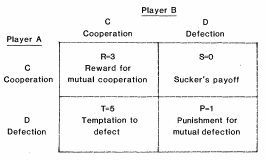
\includegraphics[scale=1]{payoffmatrix.png}
	\caption{The payoff matrix given in Axelrod and Hamilton's paper~\cite{evolution_of_cooperation}}
	\label{fig:payoffmatrix}
\end{figure}
\subsection{Strategies}

\subsection{Other Game-Theoretic Models}

\subsection{Strategies}


~\cite{arithmetics_of_mutual_help}\\
~\cite{five_rules_coop}\\
~\cite{evolution_of_cooperation}\\
~\cite{evol_indirect_image}\\
~\cite{evol_graph}\\
~\cite{multilevel_nowak}\\
~\cite{phelps_game_theoretic_analysis}\\
~\cite{spatial}\\
~\cite{heterogenous}\\
~\cite{evoldirindir}\\
~\cite{extortion}\\

%------------------------------------------------

\section{Discussion and Conclusion}
Talk about impact in real life and multi-agent systems.\\
~\cite{sticklebacks}\\
~\cite{prisonersdilemma}\\


%----------------------------------------------------------------------------------------
%	REFERENCE LIST
%----------------------------------------------------------------------------------------

\bibliography{../refs.bib}{}
\bibliographystyle{plain}

%----------------------------------------------------------------------------------------

\end{document}
